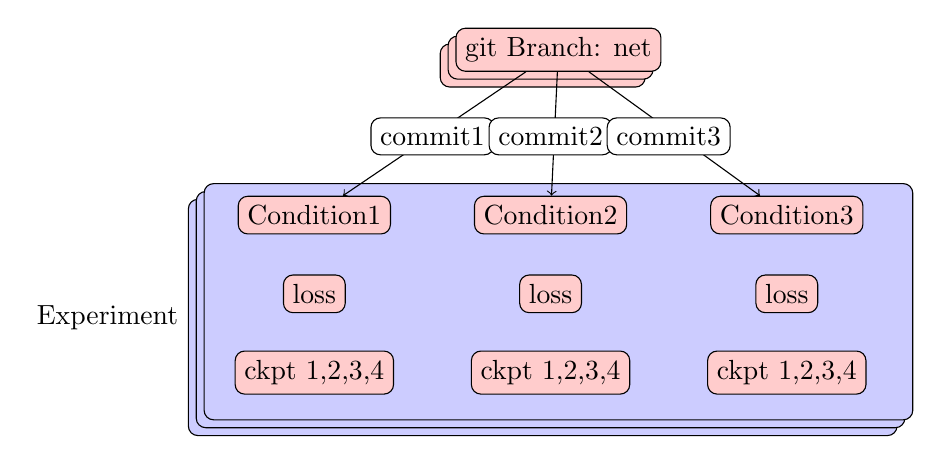
\begin{tikzpicture}
[
    level distance=4cm,
    level 1/.style={sibling distance=5cm},
    level 2/.style={sibling distance=2.5cm},
    level 3/.style={sibling distance=1cm},
    every node/.style={shape=rectangle, rounded corners=.8ex, draw, fill = red!20},
    bigbox/.style={shape=rectangle, rounded corners=.8ex, draw, fill=blue!20, minimum height=3cm, minimum width=9cm},
]
\node at (-0.1, 2.9){git Branch: net};
\node at (0,3.0){git Branch: net};
\node(branch) at (0.1, 3.1){git Branch: net};
\node at (-0.1,-0.3) [fill=blue!20, bigbox, label=west:Experiment] {};
\node at (0,-0.2) [fill=blue!20, bigbox] {};
\node at (0.1,-0.1) [fill=blue!20, bigbox] {};
\node(cond1) at (-3,1){Condition1};
\node(cond2) at (0,1){Condition2};
\node(cond3) at (3,1){Condition3};
\node(loss) at (0,0){loss};
\node(ckpt) at (0,-1){ckpt 1,2,3,4};
\node(loss) at (-3,0){loss};
\node(ckpt) at (-3,-1){ckpt 1,2,3,4};
\node(loss) at (3,0){loss};
\node(ckpt) at (3,-1){ckpt 1,2,3,4};
\draw[->] (branch) to (cond1);
\node at (-1.5, 2)[fill=white]{commit1};
\draw[->] (branch) to (cond2);
\node at (0, 2)[fill=white]{commit2};
\draw[->] (branch) to (cond3);
\node at (1.5, 2)[fill=white]{commit3};
\end{tikzpicture}